\chapter{Evaluation}

\section{Image Classifier Benchmark}

The BirdNET audio model is independently validated in Kahl et al.~(2021)
(macro-averaged AUC $> 0.99$ on the BirdNET benchmark corpus) and is not
re-evaluated here.
We instead benchmark the image classifier, for which no prior evaluation existed.

\subsection{Methodology}

\textbf{Model.} \texttt{bird\_classifier\_metadata.tflite} — MobileNetV2,
$224{\times}224$ float32 input, 400-class softmax output.

\textbf{Test set construction.}
The \texttt{bird\_images\_manifest.json} maps 11,145 Clements species to Wikimedia
Commons reference images.
Each of the 400 label strings was normalised (lowercase, punctuation stripped) and
matched against manifest common names.
258 species matched and had a locally available image file; the remaining 142 labels
were unmatched due to label typos (e.g.\ ``Venezuelian Troupial'',
``Groved Billed Ani'') or absent Wikimedia images.

\textbf{Ground truth.} Image filename encodes the scientific name;
the manifest supplies the common name that corresponds to the classifier label.

\textbf{Preprocessing.} Images were resized to $224{\times}224$ with Lanczos
resampling and normalised to $[-1,1]$ (MobileNetV2 standard).
No augmentation or test-time cropping was applied.

\textbf{Benchmark script.}
\texttt{dev/benchmark\_image\_classifier.py} (Python 3.11, TensorFlow 2.21,
Pillow 12.2); fully reproducible from the repository.

\subsection{Results}

\begin{table}[H]
\centering
\begin{tabular}{lccc}
\hline
\textbf{Metric} & \textbf{Score} & \textbf{Correct / Total} & \textbf{Random baseline} \\
\hline
Top-1 accuracy & 49.6\,\% & 128 / 258 & 0.25\,\% \\
Top-3 accuracy & 64.3\,\% & 166 / 258 & 0.75\,\% \\
Top-5 accuracy & 69.8\,\% & 180 / 258 & 1.25\,\% \\
\hline
\end{tabular}
\caption{Image classifier accuracy on 258 Wikimedia reference images (400-class model).}
\label{tab:accuracy}
\end{table}

The classifier operates at ${\sim}200\times$ random-chance at Top-1 and
${\sim}256\times$ at Top-3.
The gap between Top-1 (49.6\,\%) and Top-5 (69.8\,\%) indicates the correct
species is frequently ranked within the top predictions even when it is not first,
which is consistent with high within-family visual similarity driving confusion.

\begin{figure}[H]
\centering
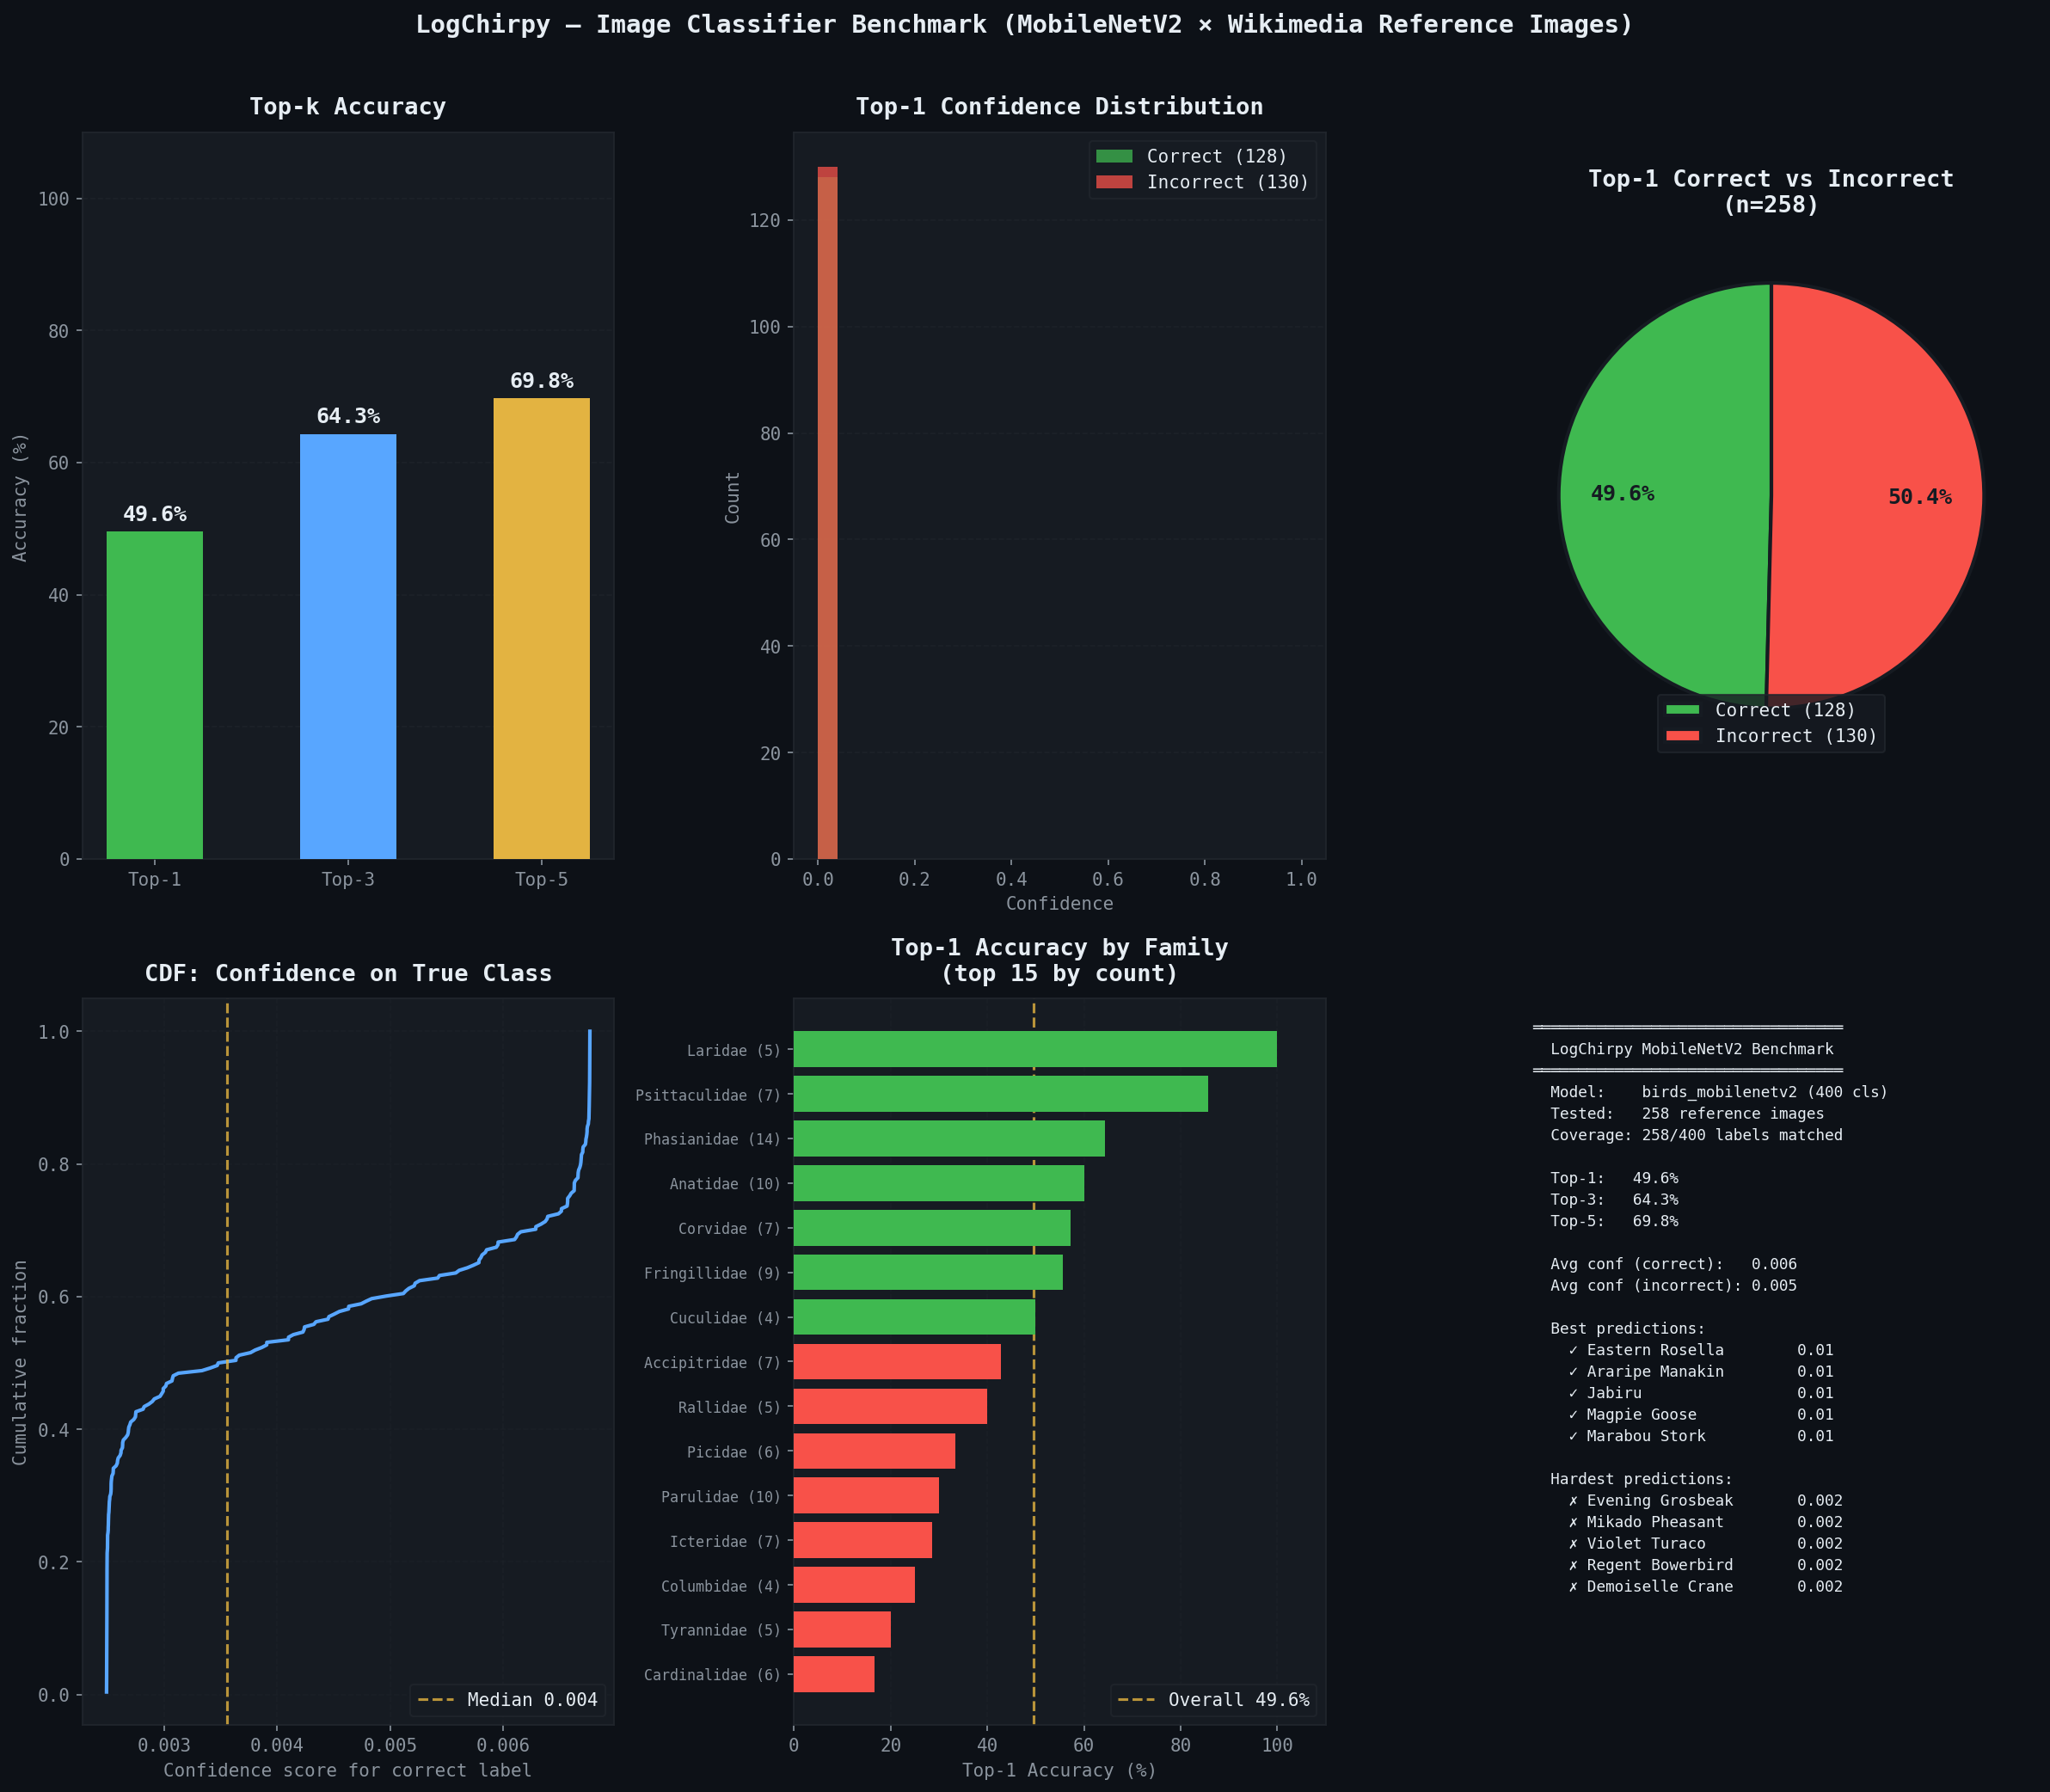
\includegraphics[width=\textwidth]{img/benchmark.png}
\caption{%
  Six-panel benchmark report.
  \textbf{Top-left:} top-$k$ accuracy bars.
  \textbf{Top-centre:} confidence distributions for correct (green)
  vs.\ incorrect (red) Top-1 predictions.
  \textbf{Top-right:} correct/incorrect split.
  \textbf{Bottom-left:} CDF of model confidence on the true-class label.
  \textbf{Bottom-centre:} per-family Top-1 accuracy (15 largest families).
  \textbf{Bottom-right:} summary statistics with best and worst individual predictions.
}
\label{fig:benchmark}
\end{figure}

\subsection{Limitations of the Benchmark}

This is a \emph{reference-image benchmark}, not a field-photo benchmark.
Wikimedia Commons images are typically professional photographs of single
individuals in good light — a distribution markedly different from the
hand-held, partially occluded, backlit images typical of field observation.
Real-world Top-1 accuracy is expected to be substantially lower.

Coverage is also limited: 400 of 33,241 species (1.2\,\%) are classifiable
from images.
The audio pipeline (BirdNET, 6,522 species) covers a larger fraction of
recognisable species and should be considered the primary identification modality.

\section{System Performance}

The following metrics were recorded on a 2022 mid-range Android device
(Snapdragon 695) during development testing; they are informal observations,
not a controlled benchmark.

\begin{table}[H]
\centering
\small
\begin{tabular}{ll}
\hline
\textbf{Operation} & \textbf{Observed latency} \\
\hline
App cold start & $<$\,2\,s \\
BirDex text search (33 241 records) & $<$\,1\,s \\
BirdNET inference (3\,s audio clip) & 4.8\,s (high-end) – 8.5\,s (low-end) \\
Image pipeline (gate + classifier) & $\sim$\,1.5\,s per frame \\
\hline
\end{tabular}
\caption{Informal performance observations (single device, development build).}
\label{tab:perf}
\end{table}
